Wind turbines and solar panels are carbon-free facilities and have become promising candidates for sustainable electricity generation. 
However, the uncertainty of wind and solar energy, which mainly comes from the difficulty of accurate long-term prediction, presents a significant challenge to traditional power scheduling system, such as infeasible or suboptimal solutions caused by day-ahead prediction errors~\cite{jabr2014robust}. The future power grids require a transformation in scheduling systems toward real-time decision-making to better utilize accurate ultra-short-term forecasts and tap the grids' flexibility. Such real-time requirement is not possible with the current computationally heavy scheduling algorithms.
In this research, we propose a reinforcement learning(RL) based real-time scheduling framework on the top of MuZero series' work.
% to leverage the \shaohuai{flexibility} of the existing grid.
Experimental results show that our approach significantly reduces renewable generation curtailment while ensuring the stable operation of a power system with high penetration of renewable energy. Moreover, our proposed approach is proved to save billions of dollars in costs for thermal generator flexibility retrofits and energy storage construction.

% The traditional day-ahead scheduling includes day-ahead unit commitments(UC) and intraday security-constrained economic dispatch(SCED). Day-ahead UC calculates the generator start/stop schedule for the following day. SCED, also called optimal power flow(OPF), calculates the optimal output power of generators in each period.
% , which minimizes operation costs, maintains grid safety constraints, and maximizes renewable energy consumption.
  
% The scheduling aims to determine the optimal output power of generators in each period that minimizes operation costs, \shaohuai{while satisfying} safety constraints.
In traditional power systems, power generation schedules are calculated by the day-ahead scheduling(DAS) program, which is often done a day or several days in advance. It consists of two stages of work. First, based on day-ahead forecasts of load and renewable generation, the start/stop schedules of thermal generators are determined by solving a so-called day-ahead unit commitment(UC) problem. Second, according to the real-time load and renewable generation, the output power of generators at each time step is optimized economically to minimize the generation costs, while satisfying the operational security constraints of power grids, which is called the intraday economic dispatch(ED) problem.
Such a procedure is practical since the power output of traditional power plants, such as fossil fuel plants, are entirely under human control, and the load prediction is also well-developed. However, due to the hardness of accurately predicting the long-term power output of increasing renewable energy sources, it is difficult to guarantee that the results of day-ahead UC are feasible.
For example, once the renewable generation is overestimated, fewer thermal generators are set in service, which could lead to insufficient power ramping capacity, load shedding caused by mismatches between power generation and load consumption, or even system failures. 
On the other hand, underestimates of renewable energy may lead to excessive thermal units in operation, which results in renewable energy curtailments.
% Therefore, to ensure system safety, operators usually maintain sufficient thermal generators in service. 
% \shaohuai{This can lead to renewable generation being curtailed if renewable energy units are generating a lot of power and the started thermal generators have reached their minimum power boundaries. Renewable power cannot be fully consumed because the power of thermal power units cannot be further reduced.} 

% % More specifically, the conventional approach to this multi-period optimization problem is to first solve unit commitment(UC) day-ahead, and then perform security-constrained economic dispatch(SCED), that is optimal power flow(OPF), in each period. 
% \shaohuai{More specifically, the conventional approach to this multi-period optimization problem could be divided into two phases. The first phase is to solve unit commitment day-ahead. The second phase performs security-constrained economic dispatch(SCED), that is, optimal power flow(OPF), which has been extensively studied in recent years~\cite{jabr2002primal,jabr2006radial,dall2016optimal}.}
% % Therefore, OPF is a fundamental optimization problem of scheduling, and has been extensively studied in recent years~\cite{jabr2002primal,jabr2006radial,dall2016optimal}. 
% However, OPF concentrates on the optimization in a single period, and generally does not consider power ramping constraints and unit start/stop interval constraints, which makes OPF quite different from the actual scheduling tasks. It is common practice to incorporate these intertemporal constraints into the unit commitment problem
% % to schedule the periods when the generators must be ready to operate and subsequently calculate the optimal dispatch by solving an OPF problem for each period
% ~\cite{jabr2012tight}. 
% However, the overestimated or underestimated renewable maximum power causes insufficient or excessive thermal generators to operate, resulting in loads being cut off or renewable power being lost. With the growing capacity of renewable energy facilities connected to grids, robust optimization methods are used to solve the day-ahead scheduling~\cite{jabr2014robust,gopalakrishnan2013global}. These methods are computationally intensive and still unable to model the probabilistic distributions of renewable generation well. To accommodate the rapid fluctuations in load and renewable energies, some studies have focused on the acceleration of OPF\cite{tang2017real,zamzam2020learning,dall2016optimal,zhou2021deep,yan2020real}. Nevertheless, many practical operating constraints are not considered yet, leading to their inapplicability to practical scheduling. 
% % Furthermore, RL is also explored to solve the unit commitment with renewable sources~\cite{de2021applying,de2022reinforcement}. However, the proposed RL methods are not used for real-time acceleration and do not take advantage of ultra-short-term forecasts.

% More specifically, the impacts of increasing renewable sources are different on the two phases of DAS. ED is a programming problem that focuses on optimization in a single period. It has been intensively studied and applied in real-world scheduling tasks~\cite{zhu2015optimization}. However, things are different in day-ahead UC, which is mathematically a multi-period mixed integer programming problem that requires day-ahead forecasts of renewable generation and load~\cite{bhardwaj2012unit}. 
% To accommodate the uncertainties proposed by prediction errors, some previous works focus on robust optimization~\cite{bertsimas2012adaptive, jabr2014robust, ruiz2009uncertainty}. These studies build on the premise that the uncertainty of renewable energy can be well modeled by probabilistic distributions, but in practice, such distributions tend to undergo some shifts over time, which introduces temporal errors and leads to infeasible solutions. Moreover, These studies have also been criticized for being computationally intensive. There are also studies that focus on the spatiotemporal dependencies between the current forecasts and the previous to reuse the UC results~\cite{cordova2018efficient}. However, the minor differences in similarity are often subject to large differences in the real scenarios, which also lead to infeasible solutions in UC. 
% Furthermore, reinforcement learning(RL) is also explored to solve UC with renewable sources~\cite{de2021applying,de2022reinforcement}. However, the proposed RL environment only takes the power balancing constraint into consideration, which is quite different from the actual scheduling tasks.

% Due to the limitations of scheduling capability, operators had to fall back on the conservative side. That is, pre-calculate a sequence of generator power plan according to the day-ahead prediction and only use the renewable energy conservatively~\cite{wood2013power}. Although real-time adjustments could be made by human operators manually, the effectiveness and safeness highly depend on their experience. As a result, 
% it is highly challenging to achieve a stable and efficient consumption of renewable generation, especially in the context of increasing renewable sources.
Under the above limitations of DAS, operators either choose to utilize renewable energy conservatively or execute flexibility retrofits to thermal generators and expand storage to increase the scheduling resources of power grids. 
Although the former requires real-time adjustments that can be done manually by human operators, the effectiveness and safety are highly dependent on their experience. The latter, while very effective in enhancing the grid's flexibility, requires a significant investment. 
Moreover, the retrofitted thermal units are likely to operate at non-economic operating conditions outside of their design specifications, instead increasing carbon emissions and costs per megawatts~\cite{chen2021flexible}. 
% The bottleneck of energy storage is that electrochemical energy storage cannot yet reach the charging/discharging power and capacity of grid-level storage, and its lifetime is also problematic. While physical-based energy storage, such as compressed air and pumped hydro storage, is highly dependent on natural geographic conditions. Either type of energy storage is very expensive to build. 
% It is very challenging to achieve stable and efficient consumption of renewable energy, especially in the context of increasing renewable energy sources. 
It is not efficient to implement future grid scheduling either by manual modifications or hardware upgrades.
% Consequently, it becomes a high priority to tap the flexibility of the existing grid.
Consequently, we want to investigate an innovative scheduling framework to deeply explore the flexibility of the existing grid.
% it is highly challenging to achieve a high share of renewable energy generation in the existing grid rather than just a high utilization level at a small installed generation capacity.

% One promising direction is exploiting the precise ultra-short-term forecasts of renewable maximum power to adjust generators in real-time, thus balancing the rapid fluctuations of renewable generation and load consumption~\cite{wu2021ultra}. 
% One promising direction is to exploit the potential of ultra-short-term forecasts since the short-term changes are small and more predictable. In such occasion, real-time decision-making can
One promising direction is incorporating precise ultra-short-term forecasts with the scheduling system to make real-time deisions.
Benefiting from the development of deep learning techniques, ultra-short-term forecasting of renewable energy generation has reached a dependable accuracy in recent years~\cite{wu2021ultra,tawn2022review}. 
However, the traditional DAS framework is difficult to schedule generation in such a short period of time.
% , which requires the entire scheduling system to transform into real-time decision-making. 
% In this way, it is possible to achieve efficient and stable operations of power grids with high penetration of renewable energy. 
Therefore, each control center requires a computationally fast algorithm that optimizes the power flow through real-time control of output power and starts/stops of generators, which is defined as the Real-Time Scheduling(RTS) problem. 
RTS is vital to utilizing the existing renewable energies and laying the foundation for broader applications in the future.  

%Due to the limitations of these prior methods, the current approach of operators to solve this non-linear, non-convex, high-dimensional, multi-objective optimization problem is to precalculate a sequence of generator power setpoints according to the precise day-ahead prediction as a power generation plan, and then make manual adjustments according to the actual conditions~\cite{wood2013power}. However, the iterative methods used to solve OPFs fall far short of real-time requirements~\cite{dommel1968optimal,sun1984optimal,jabr2002primal} and the day-ahead forecasts of renewable generation still have a large error rate.The two weaknesses have posed significant challenges to current operations on power grids with high penetration of renewable energy.

To solve the RTS problem, we first reformulate it as a sequential Markov Decision Process (MDP), inspired by some work modeling scheduling as a finite-horizon optimal control problem~\cite{chandy2010simple}. On the basis of this concept, we build a RL environment based on a provincial power grid, along with actual load and power generation data. 
\shaohuai{This environment considers the optimization of AC power flow. 
% Compared to DC power flows, AC models are more accurate but take longer to compute, which has led to less use in practical scheduling.
}
The RL agent is allowed to obtain short-term predictions of load and renewable energy maximum power from the simulator to fit the ultra-short-term prediction's setting. The parameters of the transmission lines are also the same as the actual devices. The modifications are minimally added for data security reasons. This environment is named GridSim. 

% Second, we propose an algorithm that solves the \shaohuai{scheduling} problem in real-time and takes good advantage of the ultra-short-term predictions. Our proposed algorithm deal with the unit commitments and economic dispatch problem simultaneously, maintaining a reasonable number of thermal generators in operation and keeping the grid in safety constraints while consuming renewable electricity as much as possible.
% For instance, our method achieves an average of 95\% renewable energy consumption rate. However, instead of taking 2.37 hours to run the day-ahead UC and SCED per step, our method takes only 43.2 seconds over a whole day of 288 dispatching steps, reducing the runtime by 99.5\%. Our method takes a fundamental step from pre-calculated generation arrangements to real-time interactive optimization.

On the algorithm side, 
% we formulate the problem as a sequential Markov Decision Process (MDP), inspired by some work modeling \shaohuai{scheduling} as a finite-horizon optimal control problem\cite{chandy2010simple}. However, 
instead of running an off-the-self reinforcement learning algorithm\shaohuai{Is this claim necessary? Maybe 'We refer to MuZero series' work and design....'}, we design a dedicated reinforcement learning algorithm for the Real-Time Scheduling problem, which we named GridZero. There are two major components in the GridZero algorithm. The first component is a fast neural network that can output near-optimal power grid scheduling operations. The second is a systematic search process that validates the proposed grid scheduling operations by simulating how the grid will change after the proposed operations. The search process could avoid the case when the current operation is valid but leads to future grid states that are hard to deal with. These two components are reminiscent of how an experienced power grid manager operates the grid: the operators intuitively know some good candidate controlling options according to their past experience, and then they validate the operation by further simulations. GridZero is inspired by the AlphaGo series' work, which excels at the game of Go~\cite{silver2016mastering,li2018alphago,silver2017mastering,schrittwieser2020mastering}. It seems that there is no relation between the game of Go and the power grid scheduling problem. However, we point out that both are highly complex sequential decision-making problems, and both significantly benefit from planning for the future. 

In summary, our method formulates the RTS problem as a Markov Decision Process, and we design a dedicated reinforcement learning algorithm. It avoids the load shedding of overestimating renewables and reduces the curtailment of renewable generation previously caused by underestimatings, both through the judicious use of ultra-short-term forecasts. Our method could better exploit the dispatching potential of the existing grid, and save huge amounts of costs in flexibility retrofits and storage construction. The proposed RL method also shifts the computational burdens from the iterative optimization process to an offline training process and achieves better solution quality simultaneously. Our algorithm could be one of the vital components of the future power grid that embraces renewable energies. 


%To address the RT-OPF problem, we believe that the agents should have the planning capability. RT-OPF is eventually a kind of planning-required problems, where planning based RL algorithms, such as MuZero and EfficientZero, have shown their ability by planning meticulously with a fine-grained dynamic model~\cite{schrittwieser2020mastering,ye2021mastering}.
% MBRL algorithms, such as MuZero and EfficientZero, have achieved great success in some challenging tasks such as Atari and board games by planning meticulously with a fine-grained dynamic model \cite{schrittwieser2020mastering,ye2021mastering}. 
% The planning provided by the learnable dynamic model will not be constrained by the bottleneck of communication speed.
% Compared to model-free methods, such an environmental model is beneficial for better policy learning, especially in such a planning-needed tasks. 
% The powerful policy improvements provided by precise search can help bypass the imitation learning process, which will significantly reduce the cost of producing pre-trained datasets.
%The powerful policy improvements provided by the precise search could help bypass the imitation process, which could significantly reduce the cost of producing a pretrained dataset.
% \weirui{What is model-free methods? Is there any model-free methods in OPF? What's the performance}. 
% \textcolor{red}{We pioneer the use of MBRL for solving RT-OPF problems.}
% In our paradigm \weirui{What paradigm? Mention that ours are MBRL before this}, a single computationally efficient RL agent replaces the traditional, time-expensive optimization sequence, and make rolling planning by Monte Carlo Tree Search(MCTS), which is not possible with model-free methods~\cite{zhou2020data,zhou2021deep}. Moreover, we predict the future states with the environmental model without interactions with the simulators to reduce the computation overhead. Our method reconstructs the optimization framework, and generates a super robot operator.
%The AlphaGo/AlphaZero/MuZero series has been recognized as a 'Next Generation Operator', due to the similarities between power system operational challenges and complex decision games such as Go~\cite{li2018alphago}. However, planning-based RL has not been used for solving the RT-OPF problem.
% which is a challenging task due to its non-linear dynamics, time-varying action space and multiple objectives.
% SC-OPF, in the paradigm of RL, is a challenging task due to its high dimensional time-varying action space, non-linear dynamics and multiple objectives. 

%In this work, we present an planning-capable RT-OPF algorithm GridZero and experimentally evaluate its performance on a reinforcement learning environment GridSim. The test grid of GridSim is built on a China provincial power grid. The load and renewable generation data of transections is real measured. The parameters of transmission lines are the same as real devices. GridZero learns to adjust generators to achieve a 95\% renewable consumption rate% in the test grid with high penetration of renewable energy
%, only through interactions with the power grid simulator. 
%This takes a fundamental step from pre-calculated generation arrangements to real-time interactive optimization, whose objectives and constraints are expressed as simple reward functions rather than complicated optimization paradigms.
%We demonstrate the effectiveness of our algorithm in solving unit commitments and economic dispatch simultaneously by designing hybrid actions. DRL is a promising direction for the future OPF program design. It has tremendous potential to reshape the power dispatching framework. \weirui{Add concrete contributions}

% The basic idea of GridZero (summarized in Fig.\ref{fig:how_gridzero_work}) is to predict those aspects of the future operations that related to planning. The model receives observations (active and reactive power of generators and loads, voltages and currents of lines and buses) as input and project them into hidden states. In the planning procedure, the hidden state is updated by a recurrent inference process, which receives a previous hidden state and a original action as inputs. At each recurrent step, the model generates a policy (a Gaussian distribution of power adjustment to execute), value estimation and 1-step reward prediction. GridZero is trained end-to-end with the objective of precisely estimating policy, value, reward and next hidden state. A contrastive structure is introduced to reduce the cumulative error and information loss in recurrent state prediction inspired by EfficientZero. Intuitively, GridZero can capture the key characteristics to planning in the dynamic process.

% TODO: restart from here. 

\begin{figure}[h]
  \centering
  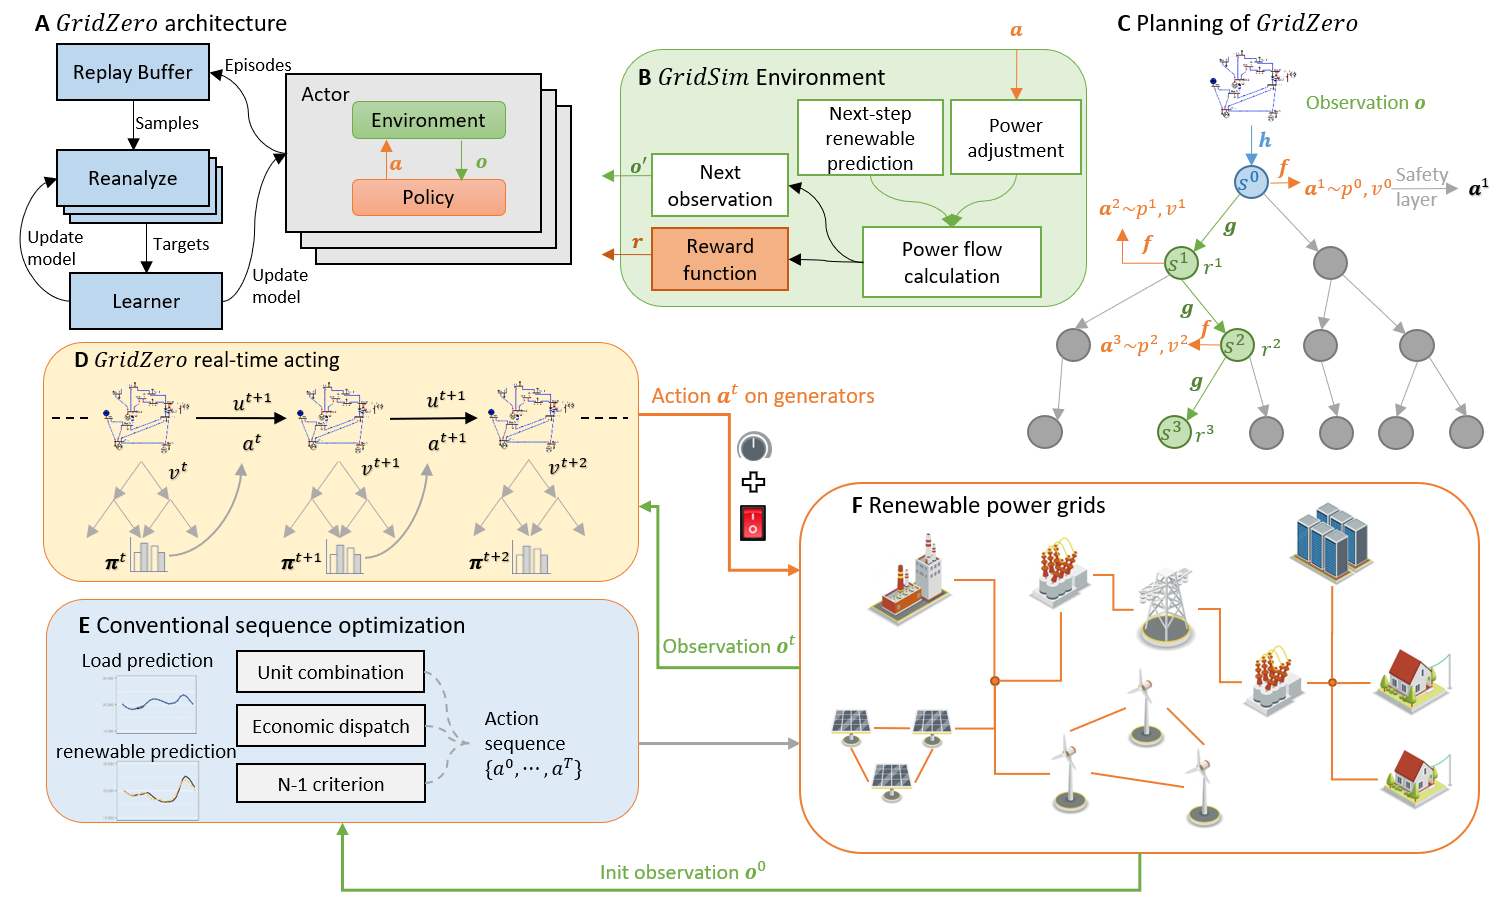
\includegraphics[width=0.85\linewidth]{fig/nature_fig1.png}
  \caption{\textbf{Representation of the components of GridZero design architecture.}
%   \weirui{The text in this figure is too small.}
  \textbf{A}. Depiction of the training architecture. GridZero sends the scheduling action to GridSim based on the current grid observation. GridSim returns the next observation and the reward based on the power flow simulation result. These state transitions are sent to the replay buffer, which feeds data to reanalyze to make targets for the learner.
  \textbf{B}. GridSim interaction loop includes next-step renewable prediction, power flow calculation, and reward function.
  \textbf{C}. Our action selection is the result of a Monte-Carlo Tree Search process. The model consists of components for representation, dynamics, and prediction. Once a previous hidden state $s^{k-1}$ and an original action $a^k$ are given, the dynamics network $g$ can output an reward estimation $r^k$ and next hidden state $s^k$. The hybrid policy $p^k$ and value estimation $v^k$ are computed by the prediction network $f$ using the hidden state $s^k$. The candidate actions $\{a^k_i\}$ are sampled from the hybrid policy $p^k$. Especially, root action candidates must be processed by the safety layer. The hidden state $s^k$ is embedded by the representation network $h$ by using the observation of the whole power grid $o^k$.
  \textbf{D}. GridZero acts in a sequential Markov decision process that outputs an action and receives an observation interactively. 
  \textbf{E}. The conventional DAS precalculates a sequence of scheduling solutions based on the precise day-ahead prediction of load consumption. However, this framework is challenged by the inaccurate day-ahead prediction of renewable generation.
%   simulates and solves three sub-problems sequentially. It finally outputs an action sequence. 
  \textbf{F}. A schematic of a power grid with renewable energy. Wind turbines, solar panels, and thermal generators work together to deliver power to the load. 
%   \textbf{G}. Performance of a whole day optimization test. GridZero achieves an average renewable consumption rate of 89.7\%.
  } 
  \label{fig:nature_fig1}
\end{figure}

% \subsection{Previous Work}
% DRL could be divided into two main directions: model-based and model-free. 


\subsection*{Real-time scheduling as an RL problem}
% DAS includes UC, a high-dimensional mixed integer programming(MIP) problem that is easily affected by the long-term prediction errors. In this case, we choose to reformulate the scheduling as a sequential Markov decision process(MDP), because this allows us to better incorporate the ultra-short-term predictions as well as the operation constraints and objectives. 
This section shows how to reformulate the RTS as an MDP and solve it. The proposed MDP incorporates the ultra-short-term predictions perfectly, as well as the operational constraints and objectives.
% The sequential process modeling could also help reduce the number of decision variables per step to decouple the computational time from the number of actual time steps. 
For better understanding, our real-time scheduling framework is illustrated in Fig.\ref{fig:nature_fig1}. There are two major phases in the approach. Our first step is to formulate the RTS problem as an MDP and create an RL environment GridSim. Second, we propose a planning capable agent GridZero that interacts with GridSim to find near-optimal policies 
% to achieve the specified objectives 
through meticulous search processes.
% The reward functions consist of specific operational objectives and constraints. The state transitions are simulated via a professional power flow analysis program. 
\subsubsection*{MDP formulation and environment design}
In the first phase, 
the MDP is modeled as follows:
\begin{enumerate}[label=(\arabic*)]
    \item Observations encode the grid operational states, including generator output power, load consumption power, line transmission power, bus voltages, etc. Observations also include the next-step prediction of renewable maximum power and load consumption.
    \item Actions are designed as combinations of continuous adjustments of generator active power output and the discrete unit starts/stops, which aims to optimize the economic dispatch and unit commitment simultaneously. In addition, the renewable generator is modeled as controllable to increase the feasible solution space. Its legal power setpoint space is $[0, P_{\text{max}}^t]$ where $P_{\text{max}}^t$ is the maximum power at step $t$. \shaohuai{Renewable energy curtailment is the difference between the actual power and the maximum power.}
    \item State transitions represent the dynamic process to the next state, and they are \shaohuai{modeled in AC power flow models and} simulated through a professional power flow analysis program. 
    \item The reward is a scalar function that measures the grid's current state under the criteria of specific constraints and objectives. It also penalizes actions that lead to undesirable states.
\end{enumerate}
% In order to depict the characteristics of future grids with high penetration of renewable energy, GridSim introduces a modified provincial power grid, SG-126, which has 126 buses, 91 loads, and 54 generators, 17 of them are renewable. The maximum generation of renewable energy accounts for more than 70\% of load consumption.

The proposed RL environment GridSim is based on the applied power flow analysis program of China Electric Power Research Institute. In order to depict the characteristics of future grids with high penetration of renewable energy, GridSim introduces a modified provincial power grid, SG-126, which has 126 buses, 91 loads, and 54 generators, 17 of them are renewable. The maximum generation of renewable energy accounts for more than 70\% of load consumption. Operational transections, including load, renewable generation data, and generator power set-points, are from actual measurements over a whole year, with data points spaced at 5-minute intervals for a total of 105,120 operational transections. Training and test datasets are separated and consist of measured transections of 2 consecutive years, which ensures that the agent is supposed to capture the essential dynamic characteristics of the grid operation instead of overfitting the training dataset. 
% GridSim reads the specified transection as an initial observation at reset and then simulates the next observations step-by-step according to actions. 
% Observations include the one-step forecasts of load consumption and renewable maximum power.


\subsubsection*{Algorithm design on the top of MuZero series}
In the second phase, we design an RL algorithm with meticulous planning processes that solves the RTS problem,
as shown in Fig.\ref{fig:nature_fig1}a,b. The proposed RL environment considers operational rules especially the thermal power ramping limitations and start/stop minimum interval constraints which are not considered in some related works~\cite{zhou2021deep,yan2020real}.

The RL algorithm learns from simulated interactions. However, purely random explorations could lead to severe consequences in a mission with such high security requirements. In the power system operation, the most important constraint is to keep power generation equal to the load consumption. More precisely, the time-varieties of renewable maximum power and load consumption make the boundaries of the action space also dynamically changes over time. To overcome the time-varying power balancing constraint, we design a safety layer and exploit the planning advantages. The safety layer adds linear modifications on the illegal actions of root nodes, and then maps them to the feasible solution space. It is necessary because violations of power balancing lead to immediate episode overs, thus no further explorations could help to learn the dynamic boundaries and policy improvements. This is common in many other similar tasks with high safety requirements. 

The search procedure to find a carefully selected action candidate is to generate a growing search tree, as shown in Fig.\ref{fig:nature_fig1}c. At each simulation, we dive to a leaf node along the most promising path, consisting of the child nodes with the highest Upper Confidence Bound (UCB) scores. Once reaching the leaf, we sample action candidates from the hybrid policy and generate new nodes to do further planning with the help of dynamics, reward, and value functions. More specifically, the observation at each root node is embedded as a vectorized hidden state by the representation function. Then a discounted future cumulative reward and a hybrid policy are correspondingly calculated by the value function and the policy function, using the vectorized hidden state as input. Once the hybrid policy is determined, the concrete action candidates, including generator power set points and on/off switchings, can be sampled from the hybrid policy. At each node, the agent could choose the most promising candidate with the highest UCB score. The reward and dynamic functions could estimate the immediate return and next hidden state if the action is selected.

% GridZero applies a search process at each step and modifies the infeasible sampled action to produce a feasible selected action and receives a reward and a next-step observation from the RL environment interactively, as shown in Fig.\ref{fig:nature_fig1}d. However, the conventional DAS solves this problem by mixed integer programming, using the original grid state, day-ahead load, and renewable generation forecasts as inputs. It pre-calculates generation arrangements of a long period in the future rather than making scheduling decisions in real-time. 
% In contrast, the prediction errors of renewable generation increase over time and can be introduced into the subsequent optimization processes, which leads to infeasible generation plans and system failures.

% Overall, our proposed method structurally reforms the day-ahead scheduling procedure into a look-ahead sequential decision process, as depicted in Fig.\ref{fig:nature_fig1}d,e. 
% The RL-driven design proposes a real-time scheduling system.
